% author: Jonah Miller
% inspired by Christian Feuersaenger

\documentclass[border=10pt]{standalone}
\usepackage{pgfplots}
\pgfplotsset{width=7.5cm,compat=1.9}

\newcommand\expr[2]{0.5*sin(20*(#1*#1+#2*#2))}

\begin{document}
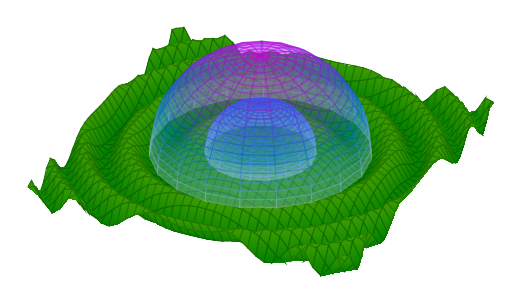
\begin{tikzpicture}
	\begin{axis}
          [
          grid=none,
          hide axis,
          axis equal,
          ]

          \addplot3[
          domain=-2*pi:2*pi,
          domain y=-2*pi:2*pi,
          surf,
          samples=40,
          shader=faceted interp,
          colormap/greenyellow,
          ] 
          {\expr{x}{y}};

        \addplot3[
        surf,
        colormap/cool,
        samples=20,
        domain=0:pi/2,
        domain y=0:2*pi,
        opacity=0.4,
        z buffer=sort
        ]
        ( {2*sin(deg(x))*cos(deg(y))},
          {2*sin(deg(x))*sin(deg(y))},
          {2*cos(deg(x))}        
        );

        \addplot3[
        surf,
        colormap/cool,
        samples=20,
        domain=0:pi/2,
        domain y=0:2*pi,
        z buffer=sort,
        opacity=0.3
        ]
        ( {4*sin(deg(x))*cos(deg(y))},
          {4*sin(deg(x))*sin(deg(y))},
          {4*cos(deg(x))}        
        );
      
	\end{axis}
\end{tikzpicture}
\end{document}